\documentclass[amsmath,longbibliography,secnumarabic,floatfix,amssymb,nofootinbib,nobibnotes,letterpaper,11pt,tightenlines,notitlepage,showkeys,showlabels]{amsart}%{revtex4-1}

\usepackage[utf8]{inputenc}
\usepackage[
style=ieee,
backend=biber]{biblatex}

\addbibresource{sources.bib}

\usepackage[top=1in, left=1in, right=1in, bottom=1in]{geometry}
\usepackage{showlabels}
\usepackage[svgnames]{xcolor}
\usepackage{latexsym, amsmath, amscd, amsthm}
\usepackage{mathrsfs}
\usepackage{tikz}
\usepackage{pgfplots}
\usepackage{graphicx}
\usepackage{brunnian}
\usepackage{mathtools}
\usepackage{hyperref}
\usepackage{algorithmicx}
\usepackage{algpseudocode}
\usepackage{enumerate}
\usepackage{setspace}

\setlength{\parskip}{.1cm}

\usetikzlibrary{decorations.markings,backgrounds,hobby}

\newcommand{\Z}{\mathbb{Z}} \newcommand{\N}{\mathbb{N}}

\newcommand{\UnkDia}{\mathcal{U}}
\newcommand{\TrefSum}{\mathcal{T}}
\newcommand{\KnotDia}{\mathcal{K}}
\newcommand{\knotdia}{\kappa}
\newcommand{\FlatKnotDia}{\mathscr{K}}
\newcommand{\KnotShad}{\FlatKnotDia}
\newcommand{\knotshad}{k}
\newcommand{\knotgrowth}{\mu_K}
\newcommand{\LinkDia}{\mathcal{L}}
\newcommand{\linkdia}{\lambda}
\newcommand{\LinkShad}{\mathscr{L}}
\newcommand{\linkshad}{\ell}

\newcommand{\PrimeLinkDia}{\mathcal{PL}}
\newcommand{\primelinkdia}{p\lambda}
\newcommand{\PrimeLinkShad}{\mathscr{PL}}
\newcommand{\primelinkshad}{p\ell}
\newcommand{\PrimeKnotDia}{\mathcal{PK}}
\newcommand{\primeknotdia}{p\kappa}
\newcommand{\PrimeKnotShad}{\mathscr{PK}}
\newcommand{\primeknotshad}{pk}


\newcommand{\ArbMaps}{\mathscr{M}}
\newcommand{\PrimeShad}{\mathscr{P}}
\newcommand{\ArbSurf}{\Sigma}
\newcommand{\ArbClass}{\mathscr{C}}
\newcommand{\ArbObj}{C}
\newcommand{\ArbSubClass}{\mathscr{D}}
\newcommand{\arbsubclass}{d}
\newcommand{\arbclass}{c}
\newcommand{\PatCount}{E}
\newcommand{\Prb}{\mathbb{P}}
\newcommand{\Shad}[1]{\tilde{#1}}
\newcommand{\FourTang}{\&}
\newcommand{\GraphOf}[1]{\Gamma(#1)}

\newcommand{\Expand}{T}
\DeclareMathOperator{\Aut}{aut}
\DeclareMathOperator{\im}{im}

\newtheorem*{conjecture}{Conjecture}
\newtheorem*{notmythm}{Theorem}
\newtheorem{theorem}{Theorem}
\newtheorem{proposition}[theorem]{Proposition}
\newtheorem{lemma}[theorem]{Lemma}
\newtheorem*{lemma*}{Lemma}
\newtheorem{corollary}[theorem]{Corollary}
\theoremstyle{definition}
\newtheorem*{definition}{Definition} 

\tikzset{->-/.style={decoration={ markings, mark=at position #1
      with {\arrow{>}}},postaction={decorate}}}

\begin{document}
%%% HEAD MATTER
\title[]{On the asymptotics of uniformly random knot diagrams} \author{Harrison Chapman}
\email{hchapman@math.uga.edu} 
\address{Department of Mathematics\\
University of Georgia, Athens GA}
% \noaffiliation{}
\date{\today}
%%%


\begin{abstract}
  We study random knotting by considering knot and link diagrams as
  decorated, (rooted) combinatorial maps on spheres, and pulling them
  uniformly from among sets of a given number of vertices $n$. We
  prove some asymptotic results and examine how quickly this behavior
  occurs in practice. En route, we show how some asymptotic laws for
  unlabeled maps apply to decorated maps as well.
\end{abstract}
\maketitle

\doublespacing
\section{Introduction}
\label{sec:intro}

\subsection{Random knotting}
\label{sec:random-knotting}

There is a dearth of models for drawing random knots; self avoiding
lattice walks \cite{Sumners_1988}, random space polygons
\cite{Cantarella_2015,Cantarella_2013}, random braid words [cite],
\emph{Petaluma} \cite{petaluma1}, et.\ al. In this paper we will
discuss the \emph{random diagram model} introduced in
\cite{CCMknotdiagrams2015} under which \emph{knot diagrams} are drawn
uniformly from the set of all diagrams with a given number of
crossings. There has been some work on sampling random
diagrams\cite{diaoernst2012pnmkt}, but the distributions
are not precisely understood.  As well, alternating knot and link
diagrams have been studied \cite{PZJasympconj2004} but little is
published about the knottiness of arbitrary random diagrams of large
size.

In this paper we begin by considering a slightly different object,
\emph{rooted diagrams}, which break symmetries (as opposed to in
). We are then able to prove that in the
limit, knot diagrams behave similarly to rooted diagrams, so that
these results carry over.

\subsection{Definitions}
\label{sec:prelimdefs}

\subsubsection{Knots, links, and tangles}
\label{sec:knotlinktangledef}

A \emph{link} is an isotopy class of embeddings of one or more circles
into $S^3$. A \emph{knot} is an isotopy class of embeddings of exactly
one circle into $S^3$. Both of the prior are considered up to
\emph{ambient isotopy} of the embedded circles. A \emph{knot diagram}
(resp. \emph{link diagram}) is a generic immersion of a
circle (resp. any number of circles) into the sphere $S^2$ (generic in
that all intersection points are double points) together with
over-under information at each double strand. The study of links and
knots is well known to be equivalent to the study of link diagrams and
knot diagrams up to the so-called
\emph{Reidemeister moves}, shown in figure~\ref{fig:reidemeister} by a
theorem of Reidemeister.
\begin{figure}[h!]
  \begin{tabular}{c@{\hspace{4em}}c@{\hspace{4em}}c}
  \centering
  \begin{tikzpicture}[every path/.style={string, very thick}, every node/.style={transform shape,
      knot crossing, inner sep=1.5pt}]
    \begin{scope}
      \node (X) at (0,0) {};
      \node (L) at (0,.7) {};
      \node (lC) at (.5,0) {};

      \node (A) at (-.5,-.5) {};
      \node (B) at (.5,-.5) {};

      \draw (A) -- (X.center);
      \draw (X.center) .. controls (X.4 north east) and (L.4 east) .. (L.center);
      \draw (X) .. controls (X.4 north west) and (L.4 west) .. (L.center);
      \draw (X) -- (B);
    \end{scope}
    \begin{scope}[xshift=.8in]
      \node (A) at (-.5,-.5) {};
      \node (B) at (.5,-.5) {};

      \node (X) at (0,.7) {};
      \node (rC) at (-.5,0) {};

      \draw (A)        .. controls (A.8 north east) and (X.4 west) .. (X.center);
      \draw (X.center) .. controls (X.4 east) and (B.8 north west) .. (B);
    \end{scope}
    \draw[<->] (lC) -- (rC);
  \end{tikzpicture}
    &
  \begin{tikzpicture}[every path/.style={string, very thick}, every node/.style={transform shape,
      knot crossing, inner sep=1.5pt}]
    \begin{scope}
      \node (X1) at (0,-.2) {};
      \node (X2) at (0,.4) {};
      \node (lC) at (.5,0) {};

      \node (A1) at (-.5,-.5) {};
      \node (A2) at (-.5,.7) {};
      \node (B1) at (.5,-.5) {};
      \node (B2) at (.5,.7) {};

      \draw (A1) -- (X1.center);
      \draw (X1.center) .. controls (X1.2 north east) and (X2.2 south east) .. (X2.center);
      \draw (X2.center) -- (A2);

      \draw (B1) -- (X1);
      \draw (X1) .. controls (X1.2 north west) and (X2.2 south west) .. (X2);
      \draw (X2) -- (B2);
    \end{scope}
    \begin{scope}[xshift=.8in]
      \node (A1) at (-.5,-.5) {};
      \node (A2) at (-.5,.7) {};
      \node (B1) at (.5,-.5) {};
      \node (B2) at (.5,.7) {};

      \node (X1) at (-.2,.1) {};
      \node (X2) at (.2,.1) {};
      \node (rC) at (-.5,0) {};

      \draw (A1) .. controls (A1.2 north east) and (X1.2 south) .. (X1.center);
      \draw (A2) .. controls (A2.2 south east) and (X1.2 north) .. (X1.center);
      \draw (B1) .. controls (B1.2 north west) and (X2.2 south) .. (X2.center);
      \draw (B2) .. controls (B2.2 south west) and (X2.2 north) .. (X2.center);
    \end{scope}
    \draw[<->] (lC) -- (rC);
  \end{tikzpicture}
      & \begin{tikzpicture}[every path/.style={string, very thick}, every node/.style={transform shape,
      knot crossing, inner sep=1.5pt}]
    \begin{scope}
      \node (lC) at (.5,0) {};

      \node (A1) at (-.6,-.2) {};
      \node (A2) at (.6,-.2) {};
      \node (B1) at (-.5,-.5) {};
      \node (B2) at (.2,.7) {};
      \node (C1) at (.5,-.5) {};
      \node (C2) at (-.2,.7) {};

      \node (X1) at (-.3,-.2) {};
      \node (X2) at (.3,-.2) {};
      \node (X3) at (0,.3) {};

      \draw (A1) -- (X1.center) -- (X2.center) -- (A2);
      \draw (B1) -- (X1);
      \draw (X1) -- (X3.center) -- (B2);
      \draw (C1) -- (X2) -- (X3) -- (C2);
    \end{scope}
    \begin{scope}[xshift=.8in]
      \node (A1) at (-.6,.4) {};
      \node (A2) at (.6,.4) {};
      \node (B1) at (-.5,.7) {};
      \node (B2) at (.2,-.5) {};
      \node (C1) at (.5,.7) {};
      \node (C2) at (-.2,-.5) {};

      \node (X1) at (-.3,.4) {};
      \node (X2) at (.3,.4) {};
      \node (X3) at (0,-.1) {};

      \draw (A1) -- (X1.center) -- (X2.center) -- (A2);
      \draw (B1) -- (X1);
      \draw (X1) -- (X3) -- (B2);
      \draw (C1) -- (X2) -- (X3.center) -- (C2);

      \node (rC) at (-.5,0) {};
    \end{scope}
    \draw[<->] (lC) -- (rC);
  \end{tikzpicture}

  \end{tabular}
  \caption{The three Reidemeister moves.}
  \label{fig:reidemeister}
\end{figure}

A \emph{$2k$-tangle} is a generic immersion of $k$ intervals and any
number of (possibly no) closed circles into $B^3$ so that the $2k$
interval ends all lie in the boundary. A \emph{$2k$-tangle diagram} is
a generic immersion of $k$ intervals and any number of closed circles
into $S^2$ together with over-under information at each double
point. In this paper, we will only discuss tangle diagrams in which
all $2k$ ends of the intervals lie in the same face of the sphere, so
that the $2k$-tangle diagram may be viewed as being an immersion into
the disk $D^2$ with the $2k$ interval ends lying in the boundary
circle.
\begin{figure}[h!]
  \centering
  \caption{A $6$-tangle diagram with 3 strands, and a $6$-tangle diagram with 4.}
  \label{fig:2ktangle}
\end{figure}

\subsubsection{Topological maps}
\label{sec:topmapdefs}

Diagrams are considered up to ``embedded graph isomorphism.'' This
precisely means that the viewpoint we should have is that of
\emph{topological maps} (in the cartographic sense) on
surfaces.

If $\ArbSurf$ is a surface, then its Euler characteristic
$\chi(\ArbSurf)$ is a topological invariant. The type $g$ of a surface
is defined by $\chi(\ArbSurf) = 2 - 2g$ (this definition agrees
precisely with the genus $g$ of orientable surfaces).

\begin{definition}
  A \emph{map with $n$ vertices} $M$ is a graph $\GraphOf M$ embedded
  on a surface $\ArbSurf$ of type $g$ so that every connected
  component of $\ArbSurf \setminus M$ is a topological disk. The
  connected components of $\ArbSurf \setminus M$ are called the
  \emph{faces} of $M$.

  A map $M$ is \emph{4-regular},
  \emph{4-valent}, or \emph{quartic} if every vertex in the underlying
  graph $\GraphOf M$ has degree 4.

  If $\ArbSurf$ is the sphere, then the map $M$ is called \emph{planar}.
\end{definition}

The concerns of symmetry complicates the study of maps. A strategy to
avoid this issue is to \emph{root} the map by picking and directing a
single edge.

\begin{definition}
  A \emph{rooted map} is a map
  together with a single edge marked with a direction, called a
  \emph{root edge}.
  
  An automorphism of a rooted map $M$ would be required to fix the
  root edge and its direction; hence $\Aut(M)$ is the trivial group.
\end{definition}

In this paper we will only consider planar maps, although by
considering maps on any oriented surface of arbitrary genus one can
arrive at \emph{virtual} diagrams. Furthermore, as each face must be a
disk, maps' underlying graphs are necessarily connected.

\begin{figure}[h!]
  \centering
  \begin{tikzpicture}[every path/.style={string, very thick}, every node/.style={transform shape,
      knot crossing, circle, fill=black, inner sep=2pt}]
    \begin{scope}
      \node (A) at (-1,0){};
      \node (B) at (0,1) {};
      \node (C) at (1,0) {};

      \node (D) at (-1,-2) {};
      \node (E) at (1,-2) {};

      \node (X) at (-2,-2) {};
      \node (Y) at (0, -1) {};
      \node (Z) at (-2,-1) {};

      \draw (A) -- (B) -- (C) -- (E) -- (D) -- (A);
      \draw (X) -- (D);
      \draw (A) -- (C);

      \draw (D) edge[out=90,in=180] (Y);
      \draw (D) edge[out=0,in=270] (Y);
      \draw (Y) edge[out=90,in=0,looseness=20] (Y);

      \draw (A) -- (Z);
      \draw (Z) edge[out=180+45,in=90+45,looseness=20] (Z);
      \draw (A) edge[out=90,in=180,looseness=20] (A);
    \end{scope}
    \begin{scope}[xshift=2in]
      % \draw[help lines,step=8pt] (-2,-2.6) grid (2.7,1);
      \useasboundingbox (-2,-2.6) rectangle (2.7,1);
      \node (A) at (-.8,0){};
      \node (B) at (0,-1) {};
      \node (C) at (.8,0) {};
      \node (D) at (0,-2) {};

      \node (Z) at (1.75,-1) {};

      \draw (A) -- (C);
      \draw (A) edge[out=75,in=105,looseness=1.3] (C);
      \draw (A) -- (B);
      \draw (C) -- (B);
      \draw (B) edge[out=180+45,in=90+45] (D);
      \draw (B) edge[out=270+45,in=45] (D);
      \draw (D) edge[out=180+45,in=180,looseness=2] (A);
      \draw (D) edge[out=270+45,in=-90,looseness=1.3] (Z);
      \draw (Z) edge[out=90,in=0,looseness=1.3] (C);
      \draw (Z) edge[out=-45,in=45,looseness=20] (Z);
    \end{scope}
  \end{tikzpicture}
  \caption{Two planar maps. The map on the right is in the class of knot shadows.}
  \label{fig:egplanarmaps}
\end{figure}

\begin{figure}[h!]
  \centering
  % \includegraphics[width=2in]{dual_to_fig8twist}
  \begin{tikzpicture}[every path/.style={string, thick, gray}, every node/.style={transform shape,
      knot crossing, circle, fill=gray, inner sep=2pt}]
    \begin{scope}
      % \draw[help lines,step=.2] (-2,-2.6) grid (3,1.2);
      \useasboundingbox (-2,-2.6) rectangle (2.7,1.2);
      \node (A) at (-.8,0){};
      \node (B) at (0,-1) {};
      \node (C) at (.8,0) {};
      \node (D) at (0,-2) {};

      \node (Z) at (1.75,-1) {};

      \draw (A) -- (C);
      \draw (A) edge[out=75,in=105,looseness=1.3] (C);
      \draw (A) -- (B);
      \draw (C) -- (B);
      \draw (B) edge[out=180+45,in=90+45] (D);
      \draw (B) edge[out=270+45,in=45] (D);
      \draw (D) edge[out=180+45,in=180,looseness=2] (A);
      \draw (D) edge[out=270+45,in=-90,looseness=1.3] (Z);
      \draw (Z) edge[out=90,in=0,looseness=1.3] (C);
      \draw (Z) edge[out=-45,in=45,looseness=20] (Z);
    \end{scope}
    \begin{scope}[every path/.style={string, very thick, black}, every
      node/.style={transform shape, knot crossing, circle, fill=black,
        inner sep=2pt}]
      \useasboundingbox (-2,-2.6) rectangle (2.7,1.2);
      \node (a) at (0,.4) {};
      \node (b) at (0,-.4) {};
      \node (c) at (-.8,-1) {};
      \node (d) at (.8,-1) {};
      \node (e) at (0,-1.5) {};
      \node (f) at (2.2,-1) {};
      \node (o) at (1.7, .4) {};

      \draw (a) -- (b) -- (c) -- (e) -- (d) -- (b);
      \draw (a) -- (o) -- (f);
      \draw (d) -- (o);
      \draw (d) edge[out=-80,in=0,looseness=3.8] (o);
      \draw (c) edge[out=150,in=120,looseness=1.5] (o);
    \end{scope}
  \end{tikzpicture}
  \caption{Planar quadrangulation which is dual to a knot shadow.}
  \label{fig:dualquadeg}
\end{figure}

Maps have a well defined notion of \emph{dual map}; a map $M = (V,
E, F)$ has dual $M^* = (F, E^*, V)$, where there is an edge $(f_1,
f_2) \in E^*$ if $f_1$ is adjacent to $f_2$ in $M$ (faces are adjacent
if they share an edge on their boundaries). The dual graph of a
4-regular map is a \emph{quadrangulation}, i.e.\ a map for which every
face has four bounding edges. A map is \emph{simple} if it contains no
parallel edges or self loops (its underlying graph is simple). Given a
rooted map $M$, its dual is rooted as follows. Let $\rho$ be the root
edge of $M$ pointing from $v_1$ to the root vertex $v_2$ be adjacent
to the face $f_1$ and the root face $f_2$. Then $(f_1, f_2)$ is the
dual root edge and directed from $f_1$ to $f_2$, and $f_2$, $v_2$ are
the dual root vertex and root face, respectively (and the dual of a
dual rooted map is the original rooted map).

Maps have a notion of substructure,

\begin{definition}
  A map $P$ is a \emph{submap} of a larger (possibly rooted) map $M$
  if there exists a cycle of $k$ (possibly repeated) edges in $M$ so
  that one of the two halves of $M$ separated by the cycle is
  identical to $P$.
\end{definition}

\subsubsection{Diagrams and shadows}
\label{sec:shadowdefs}

From here on, maps, shadows, and diagrams will be assumed rooted
unless otherwise noted. Notice that we will use the word
\emph{crossings} to refer to the vertices of shadows and diagrams.

\begin{definition} 
  A \emph{map decorated by a set $S$}, $(M, s)$ is a (possibly unrooted)
  map $M$ together with a mapping $s: V(M) \to S$ which associates to
  each vertex of $M$ an element of $S$.

  A \emph{(unrooted) link shadow with $n$ crossings} is a 4-regular
  (unrooted) planar map of $n$ vertices. We will denote by
  $\LinkShad_n$ the set of all $n$-crossing link shadows.

  A \emph{(unrooted) link shadow with $n$ crossings} is a 4-regular
  (unrooted) planar map decorated with $\{+,-\}$, i.e. a choice of
  over-under strand information at each vertex. We will denote the set
  of $n$-crossing link diagrams by $\LinkDia_n$.
\end{definition}

Indeed, $\LinkShad_n$ is just another name for the class of 4-regular
planar maps in $n$ vertices; furthermore, the class of rooted planar
quadrangulations is dual to $\LinkShad_n$.  Hence, the class
$\LinkShad$ of link shadows has been counted
exactly~\cite{chapman2011surveys}. If $\linkshad_n = |\LinkShad_n|$,
then:
\[ \linkshad_n = \frac{2(3^n)}{(n+2)(n+1)}\binom{2n}{n}
\mathop{\sim}\limits_{n \to \infty} \frac{2}{\sqrt\pi}12^nn^{-5/2}. \]
From this the exact counts of link diagrams can be determined
as well. If $\linkdia_n = |\LinkDia_n|$, then
\[ \linkdia_n = \frac{2^{n+1}(3^n)}{(n+2)(n+1)}\binom{2n}{n}
\mathop{\sim}\limits_{n \to \infty} \frac{2}{\sqrt\pi}24^nn^{-5/2}. \]

\begin{figure}[h!]
  \centering
  % \includegraphics[height=1.4in]{planar_maps_rooted_ex}
  \begin{tikzpicture}[every path/.style={string, very thick}, every node/.style={transform shape,
      circle, fill=black, inner sep=2pt}]
    \begin{scope}[decoration={markings, mark=at position 0.5 with
        {\arrow{>}}}] \node (A) at (-1,0){}; \node (B) at (0,1) {}; \node (C)
      at (1,0) {};

      \node (D) at (-1,-2) {}; \node (E) at (1,-2) {};

      \node (X) at (-2,-2) {}; \node (Y) at (0, -1) {}; \node (Z) at
      (-2,-1) {};

      \draw (A) -- (B) -- (C) -- (E) -- (D) -- (A); \draw (X) -- (D);
      \draw (A) -- (C);

      \draw (D) edge[out=90,in=180] (Y); \draw (D) edge[out=0,in=270]
      (Y); \draw (Y) edge[out=90,in=0,looseness=20] (Y);

      \draw (A) -- (Z); \draw (Z)
      edge[postaction={decorate},out=180+45,in=90+45,looseness=20] (Z);
      \draw (A) edge[out=90,in=180,looseness=20] (A);
    \end{scope}
    \begin{scope}[xshift=2in,decoration={markings, mark=at position
        0.5 with {\arrow{<}}}] %\draw[help lines,step=8pt] (-2,-2.6) grid
      (2.7,1); \useasboundingbox (-2,-2.6) rectangle (2.7,1); \node (A) at
      (-.8,0){}; \node (B) at (0,-1) {}; \node (C) at (.8,0) {}; \node (D)
      at (0,-2) {};

      \node (Z) at (1.75,-1) {};

      \draw (A) -- (C); \draw (A) edge[out=75,in=105,looseness=1.3]
      (C); \draw (A) -- (B); \draw (C) -- (B); \draw (B)
      edge[out=180+45,in=90+45] (D); \draw (B) edge[out=270+45,in=45] (D);
      \draw (D) edge[out=180+45,in=180,looseness=2] (A); \draw (D)
      edge[out=270+45,in=-90,looseness=1.3] (Z); \draw (Z)
      edge[postaction={decorate},out=90,in=0,looseness=1.3] (C); \draw (Z)
      edge[out=-45,in=45,looseness=20] (Z);
    \end{scope}
  \end{tikzpicture}
  \caption{Two rooted planar maps. The map on the right is in the
    class of rooted knot shadows.}
  \label{fig:egrootedplanarmaps}
\end{figure}

Restricting the number of ``link components'' complicates counting.

\begin{definition} 
  A \emph{link component} of a (possibly unrooted) link shadow or
  diagram $D$ is an equivalence class of edges modulo meeting across a
  vertex in $D$

  A \emph{(unrooted) knot shadow} is a (unrooted) link shadow which
  consists of precisely one link component. The class of knot
  shadows with $n$ crossings is denoted by $\KnotShad_n$.

  A \emph{(unrooted) knot diagram} is a (unrooted) link diagram which
  consists of precisely one link component. The class of knot
  shadows with $n$ crossings is denoted by $\KnotDia_n$.
\end{definition} 

Knot shadows $\KnotShad_n$ represent a curious, small
subclass of $\LinkShad_n$. Indeed, exact counts for $\knotshad_n =
|\KnotShad_n|$ and $\knotdia_n = |\KnotDia_n|$ are
not known except by experiments and conjectures\cite{PZJasympconj2004}

\begin{conjecture}[Schaeffer-Zinn Justin 2004]
  There exist constants $\knotgrowth$ and $c$ such that
  \[\frac{\knotdia_n}{2^n} = \knotshad_n \mathop{\sim}\limits_{n \to \infty} c\knotgrowth^n \cdot
  n^{\gamma - 2},\]
  where 
  \[\gamma = -\frac{1 + \sqrt{13}}{6},\]
  and $\knotgrowth \approx 11.4...$.
\end{conjecture}

Finally, we can define tangles using maps.

\begin{definition}
  A \emph{(unrooted) $2k$-tangle shadow} is a (unrooted) planar map
  with $2k$ degree 1 \emph{leg vertices} and any number of 4-valent vertices. We
  will only consider tangle shadows in which all $2k$ leg vertices lie
  on the same ``exterior'' face. In this case, the shadow can be
  viewed as embedded in $D^2$ with leg vertices embedded in $\partial
  D^2$.

  A \emph{(unrooted) $2k$-tangle diagram} is a (unrooted) $2k$-tangle
  shadow decorated (at non-leg vertices) with signs $\{+,-\}$. We
  restrict ourselves to tangles which can be embedded into the disk.

  A tangle shadow (resp. diagram) $T$ is \emph{contained} in a link shadow
  (diagram) $D$ if there exists some disk $B$ on the surface into
  which $D$ is embedded such that
  \begin{enumerate}
  \item The boundary $\partial B$ intersects no vertices of $D$,
  \item The boundary $\partial B$ intersects edges of $D$ either
    transversally or not at all, and
  \item The interior of the intersection $B \cap D$ is isomorphic to
    the interior of $T$.
  \end{enumerate}
\end{definition}

Rooted (knot or link) diagrams are equivalently viewed as \emph{two-leg diagrams} or
\emph{2-tangle diagrams} as illustrated below.
\begin{figure}[h!]  \centering
  \begin{tikzpicture}[every path/.style={string, very thick}, every node/.style={transform shape,
      knot crossing, inner sep=1.5pt}]
    \begin{scope}[xshift=-1.5in] \node (tl) at (-.7,0) {}; \node (tr)
      at (.7,0) {}; \node (tc) at (0,1) {}; \draw (tl) .. controls (tl.4
      north east) and (tc.4 south west) ..  (tc.center); \draw (tc.center)
      .. controls (tc.8 north east) and (tr.8 north east) .. (tr); \draw
      (tr) .. controls (tr.4 south west) and (tl.4 south east)
      .. (tl.center); \draw (tl.center) .. controls (tl.8 north west) and
      (tc.8 north west) .. (tc); \draw (tc) .. controls (tc.4 south east)
      and (tr.4 north west) .. (tr.center); \draw[->-=.5] (tr.center)
      .. controls (tr.16 south east) and (tl.16 south west) .. (tl);
    \end{scope}

    \begin{scope}[xshift=1.5in] \node (tl) at (-.7,0) {}; \node (tr)
      at (.7,0) {}; \node (tc) at (0,1) {}; \node (el) at (-1.7,0) {}; \node
      (er) at (1.7,0) {}; \draw[>-] (el.center) .. controls (el.4 east) and
      (tl.4 south west) .. (tl); \draw (tl) .. controls (tl.4 north east)
      and (tc.4 south west) ..  (tc.center); \draw (tc.center) .. controls
      (tc.8 north east) and (tr.8 north east) .. (tr); \draw (tr)
      .. controls (tr.4 south west) and (tl.4 south east) .. (tl.center);
      \draw (tl.center) .. controls (tl.8 north west) and (tc.8 north west)
      .. (tc); \draw (tc) .. controls (tc.4 south east) and (tr.4 north
      west) .. (tr.center); \draw[->] (tr.center) .. controls (tr.4 south
      east) and (er.4 west) .. (er.center);
    \end{scope} \draw[<->] (-1.6,.3) -- (1,.3) node[text
    width=3cm,text centered,midway]{cut/splice root edge};
  \end{tikzpicture}
  \caption{A rooted diagram of a trefoil, and its equivalent two-leg diagram}
  \label{fig:treflegs2}
\end{figure}

As a key portion of this paper, we will describe how the tools
presented can be applied to other classes of diagram objects. To
demonstrate this, we will prove the results for prime diagrams as
well;

\begin{definition}
  A (possibly unrooted) shadow $D$ is \emph{prime} if it has more than
  $1$ vertex and is not $2$-edge-connected, i.e.\ there is no way to
  disconnect $\GraphOf D$ by removing 2 edges. A shadow which is not
  prime is \emph{composite}.

  A rooted shadow is \emph{two-leg-prime} if it cannot
  be disconnected by removing two edges, \textit{one being the root
    edge}. 

  Diagrams are (two-leg-)prime if their underlying shadow
  structure is.
\end{definition}

We will denote by $\PrimeLinkShad_n$ the set of prime link shadows,
$\PrimeKnotShad_n$ the set of prime knot shadows,
$\PrimeLinkDia_n$ the set of prime link diagrams, $\PrimeKnotDia_n$
the set of prime knot diagrams, and
$\primelinkshad_n$, $\primeknotshad_n$, $\primelinkdia_n$, and $\primeknotdia_n$ their respective cardinalities.

\begin{figure}[h!]  \centering
  \includegraphics[height=1.5in]{2leg_vs_reg_prime}
  \caption{A composite shadow which is two-leg-prime (left). A shadow
    which is not two-leg-prime (right). }
  \label{fig:prime2legprime}
\end{figure}

Again, the counts of prime link shadows and prime link diagrams are
known precisely. Exact counts are known from their
bijection with simple quadrangulations~\cite{AlbenqueSQT};
\[ \frac{\primelinkdia_n}{2^n} = \primelinkshad_n = \frac{4(3n)!}{n!(2n + 2)!}.\]

% There is a bijection between blossom trees and rooted link shadows.

% \begin{proposition}
%   There is a consistent way to order the components of a rooted link
%   shadow. There is a consistent way to index the vertices of a rooted
%   link shadow. There is a consistent way to index and orient the edges
%   of a rooted link shadow so that the directed edges meet head-to-tail
%   across the vertices of the shadow.
%   \label{prop:canonicalori}
% \end{proposition}

% \begin{proof}
%   Let $L$ be a rooted link shadow. Begin by labelling the edges of $L$
%   with the link component in which they lie. Index the root vertex and
%   the root edge by 1.
% \end{proof}

% \begin{corollary}
%   There is a consistent way to order and orient the components of a
%   rooted link diagram. There is a consistent way to index the
%   crossings of a rooted link diagram. There is a consistent way to
%   index the edges of a rooted link diagram. These are the same as
%   those for the underlying shadow.
% \end{corollary}

% \begin{proof}
%   These are all induced on the diagram from its shadow.
% \end{proof}

% \begin{corollary}
%   Rooted link diagrams are in bijection with rooted link shadows
%   labelled with $S = \{+, -\}$.
%   \label{cor:linkdiaaresshadows}
% \end{corollary}

% \begin{proof}
%   Given a rooted link diagram, there is a consistent orientation of
%   its components. There is hence a labelling of the underlying rooted
%   shadow with $S = \{+, -\}$ (they are the standard crossing signs). This
%   process is reversible since the consistent component orientation for
%   the diagram is identical to that of the shadow.
% \end{proof}

\subsection{Result summary}
\label{sec:result-summary}

The primary goal of this paper is to prove the following result for
unrooted knot diagrams:

\begin{theorem}
  Almost all unrooted knot diagrams are unknotted, i.e. they are in
  the same equivalence class as the unknoy $0_1$.
\end{theorem}

\section{Asymptotic structure theorems for diagrams}
\label{sec:structure}

\subsection{The Frisch-Wasserman-Delbr\"uck conjecture}
\label{sec:fwdconj}

\newcommand{\MapClass}{\mathscr{M}}

On the topic of DNA topology, Frisch and Wasserman\cite{Frisch_1961}
and Delbr\"uck\cite{delbruck1962ams} separately conjectured;

\begin{conjecture}[Frisch-Wasserman 1961, Delbr\"uck 1962]
  As the size $n$ of a circle embedded in space increases, the
  probability that the circle is knotted tends to 1.
\end{conjecture}

The conjecture was originally posed in the view of self-avoiding
lattice polygons (SAPs), where size refers to the number of steps.
We ask a similar question here for knot
diagrams: \emph{Is a knot diagram with $n$ crossings almost certainly
  knotted as $n$ tends to infinity}?

For SAPs on the lattice, the conjecture was proved in the
affirmative decades later by Sumners and
Whittington\cite{Sumners_1988} who made use of Kesten's pattern
theorem\cite{Kesten_1964,Kesten_1963} which states that patterns,
(relatively) short walk configurations, appear linearly often in long
self-avoiding walks.

We make use of a similar strategy: theorem 2 in \cite{Bender1992104}
provides a pattern theorem for knot and link shadows, provided a
strategy of attaching a desired pattern. However, care is required in
the case of knot or link \emph{diagrams}, in which each vertex takes a
value in the set $\{+, -\}$. In fact, we turn our attention to the
dual case in which \emph{faces} are labelled with an arbitrary set.

\subsection{Tangles and the pattern theorem}
\label{sec:patternthm}

\begin{theorem}Let $S$ be a set and $\MapClass$ be some class of
  decorated-maps on a surface of type $g$ and let $P$ be a planar
  decorated map
  with boundary that can be found as a submap of maps in
  $\MapClass$. Let $M(x)$ be the generating function by number of
  edges for $\MapClass$. Let $H(x)$ be the generating function by
  number of edges for those maps $M$ in $\MapClass$ that contain
  less than $ce(M)$ pairwise disjoint copies of $P$. Suppose that we
  can embed $P$ in a possibly larger rooted planar labeled map with
  boundary $Q$ and attach copies of $Q$ to each map $K$
  counted by $H(x)$ in such a way that
  \begin{enumerate}
  \item for some fixed positive integer $k$, at least $\lfloor e(K)/k \rfloor$ possible
    non-conflicting places of attachment exist,
  \item only $S$-maps in $\MapClass[S]$ are produced,
  \item for any map produced as such we can identify the copies of $Q$ that have been added and they
    are all pairwise disjoint, and
  \item given the copies that have been added, the original map and associated places of attachment
    are uniquely determined.
  \end{enumerate} If $1 > c > 0$ is sufficiently small, then $r(M) < r(H)$. The maps may be rooted or
  not.
  \label{thr:weakpattern}
\end{theorem}

The method of attachment is vague, but flexible. We will provide some examples which we use in our
results for knot diagrams. The proof extends the proof of the original theorem for maps, and makes
use of a lemma:


\begin{lemma*}[\cite{Bender1992104}, lemma 3]
 If
 \begin{enumerate}
 \item $F(z) \ne 0$ is a polynomial with non-negative coefficients and $F(0) = 0$,
 \item $H(w)$ has a power series expansion with non-negative coefficients and $0 < r(H) < \infty$,
 \item for some positive integer $k$ the linear operator $\mathscr{L}$ is given by $\mathscr{L}(w^n)
   = z^n(F(z)/z)^{\lfloor n/k \rfloor}$, and
 \item $G(z) = \mathscr{L}(H(w))$,
 \end{enumerate}
 then $r(H)^k = r(G)^{k-1}F(r(G))$.
\end{lemma*}

The proof of the theorem then remains almost unchanged from the original theorem, although care will
be necessary in defining attachment.

\begin{proof}[Proof of theorem \ref{thr:weakpattern}.]
  Let $G(z)$ be the generating function which counts $S$-maps $\mathscr{G}[S]$ which are the
  result of attaching some number between $0$ and $\lfloor n/k \rfloor$ copies of $Q$ to $S$-face
  maps $\mathscr{H}[S]$ counted by $H(x)$. The method of
  attachment leads to the relation $G(z) = \mathscr{L}(H(w))$, where $F(z) = z + z^q$ and $q$ is the
  number of edges added when a copy of $Q$ is attached, as
  \[ G(z) = \sum_{X \in \mathscr{G}[S]}{z^{e(X)}} = \sum_{Y \in \mathscr{H}[S]}{z^{e(Y)}\left( 1 +
      z^{q-1} \right)^{\lfloor n/k \rfloor}} = \mathscr{L}(H(w)).\]
  Let $g_n$ be the coefficients of $G(z)$.

  Suppose $M \in \MapClass[S]$ contains $m$ copies of $Q$. By property
  (3) of our attachment, $m \le n$. If $M$ had been produced from some
  $S$-map $K$ in $\mathscr{H}[S]$ by our attachment process, we can
  find all possible $K$ by removing at least $m - cn$ copies of $Q$
  from $M$. It is possible to bound from above the number of ways to
  do this by
  \[ \sum_{j \ge m-cn}{\binom m j} = \sum_{k < cn}{\binom m k} <
  \sum_{k < cn}{\binom n k} \le {n\binom n{cn}} \le
  \frac{n(ne)^{cn}}{{cn}^{cn}} = n\left(\frac ec\right)^{cn} =: t_n.\]
  If $M(x) = \sum{m_nx^n}$, then $m_n \ge g_n$ and $t_n > 1$ for
  sufficiently large $n$, so $m_n \ge g_n/t_n$. Hence,
  \[1/r(M) \ge \limsup_{n \to \infty}{(g_n/t_n)^{1/n}} = \lim_{n \to \infty}{(t_n)^{-1/n}}\limsup_{n
    \to \infty}{(g_n)^{1/n}} \ge (c/e)^c/r(G).\]
  By the prior lemma, $r(H)^k = r(G)^k(1 + r(G)^{q-1})$ so that
  \[ r(H)/r(M)\ \ge (1 + r(G)^{q-1})^{1/k} (c/e)^c. \]
  As $\lim_{c \to 0^+}{(c/e)^c} = 1$ and $r(G)^k(1 + r(G)^{q-1}) = r(H)^k \ge 1/12^k$, it follows
  that $r(H)/r(M) > 1$ for sufficiently small $c$, completing the proof of the theorem.
\end{proof}

The conclusion is about radii of convergence of two power series, and may appear an esoteric
result. However, application of the Cauchy-Hadamard theorem, together with one additional
hypothesis, gives a more familiar tune:

\begin{corollary}[\cite{Bender1992104}]
  Suppose all of the hypotheses of theorem \ref{thr:weakpattern} and additionally that $\MapClass[S]$
  grows smoothly, i.e.\ that $\lim_{n\to\infty}{m_n^{1/n}}$ exists. Then there exists constants $c >
  0$ and $d < 1$ and $N > 0$ so that for all $n \ge N$,
  \[ \frac{h_n}{m_n} < d^n. \]
  I.e., the pattern $P$ is \emph{ubiquitous}.
  \label{thr:strongpattern}
\end{corollary}

Because of Euler's formula, the number of vertices, edges, or faces in a link shadow or planar
quadrangulation is entirely determined by choosing any one cardinality. Hence, we can size shadows
by the number of vertices and still keep the above results.

\subsubsection{Smooth growth}
\label{sec:smooth-growth}

The theorem in the prior section by itself does not sufficiently prove \emph{ubiquity} as required
to prove asymmetry. One may worry about bad cases; e.g., one in which . Indeed, we require that the
class of maps \emph{grow smoothly}, i.e.\ that (for $m_n = |\MapClass_n|$) the limit
\[ \lim_{n\to\infty}{m_n^{1/n}} \] exists.

Bender, et al.\ \cite{Bender1992104} give a powerful proof strategy for proving smooth growth of a
sequence. We adapt that to prove the following theorem.

\begin{theorem}
  Let $\ArbClass$ be a class of combinatorial objects with generating
  function $\sum_{n=0}^{\infty}{\arbclass_n~z^n}$; let the radius of
  convergence of the OGF be $r$, and $\ArbSubClass$ some other class
  with generating function
  $\sum_{n=0}^{\infty}{\arbsubclass_n~z^n}$. Suppose that $0 > r \le
  1$ and let $C_i > 0$ and $1-r>\delta>0$ be arbitrary.

  Suppose there is a composition operation $\times$ on elements $A, B
  \in \ArbClass \cup \ArbSubClass$ so that,
  \begin{enumerate}
  \item $A \times B \in \ArbClass$,
  \item there exists some fixed $k \in \Z_{\ge 0}$ so that $|A \times
    B| = |A| + |B| + k$, and
  \item given any $C \in \ArbClass$, there is at most one maximal
    factorization $D_1 \times D_2 \times \cdots \times D_s = C$ with $D_i
    \in \ArbSubClass$.
  \end{enumerate} Suppose there exists $R \ge 0$ so that for $n \ge R$
  there exists $\ell \in \Z_{\ge 0}$ and maps $\psi_0: \ArbClass_n
  \hookrightarrow \ArbSubClass_{n+\ell}$ and $ \psi_1: \ArbClass_n
  \hookrightarrow \ArbSubClass_{n+\ell+1}$. Then the limit
  \[ \lim_{n\to\infty}{\arbclass_n^{1/n}} \] exists.
\end{theorem}

It is known that there are at most $12^n$ planar maps, and so in our cases we will always have $r
\ge 1/12$.

\begin{proof}
  For some classes which can be shown to be subadditive, this follows
  by Fekete's lemma. However, there is a framework to show this result
  in more complicated cases.

The proof breaks down into 3 steps;
\begin{enumerate}
\item \emph{Show that there exists some $n \ge 0$ with $\arbclass_n > C_1(r + \delta)^{-n}$.} This
  step follows from the Cauchy-Hadamard theorem, which says that
  \[ \limsup_{n\to\infty}{\arbclass_n^{1/n}} = r^{-1}. \]

  By the definition of lim sup, we have that if $a < r^{-1}$, then for
  any $M \ge R$ we have that there is some $n \ge M$ with
  $\arbclass_n^{1/n} > a$. For instance, we know that $(r +
  \delta/2)^{-1} < r^{-1}$, hence for any $M$ we have some $n \ge M$
  with $\arbclass_n > (r+\delta/2)^{-n}$. Notice now that as
  \[ \left( \frac{r+\delta}{r + \delta/2} \right) > 1, \] there must
  be some $M \ge R$ so that for all $m \ge M$
  \[ \left( \frac{r+\delta}{r + \delta/2} \right) > C_1^{1/m}, \text{
    implying that } (r + \delta/2)^{-m} > C_1(r + \delta)^{-m}, \]
  whence we then have (by lim sup) some $n \ge M$ with $c_n >
  (r+\delta/2)^{-n} > C_1(r+\delta)^{-n}$.
\item \emph{Show that there exists some $m \ge 0$ with $\arbsubclass_m
    > C_2(r + \delta)^{-m}$ and $\arbsubclass_{m+1} > C_2(r +
    \delta)^{-(m+1)}$.} Notice that $(r + \delta) < 1$ and so for any
  $m \ge 0$, $(r + \delta)^{-m} < (r+\delta)^{-(m+1 )}$. As there
  exist injections $\psi_0, \psi_1$ from $\ArbClass_n$ into
  $\ArbSubClass_{n+\ell}$ and $\ArbSubClass_{n+\ell+1}$, setting $m =
  n + \ell$ and $C_1 = C_2(r+\delta)^{-(m+n-1)}$ we have that
  \[ \arbsubclass_m \ge |\im \psi_0| = \arbclass_n >
  C_1(r+\delta)^{-n} = C_2(r+\delta)^{-(m+1)} > C_2(r+\delta)^{-m} \]
  and
  \[ \arbsubclass_{m+1} \ge |\im \psi_1| = \arbclass_n > C_1(r+\delta)^{-n} =
  C_2(r+\delta)^{-(m+1)}. \]
\item \emph{Show that there exists some $N$ so that for any $n \ge N$,
    $\arbclass_n > (r + \delta)^{-n}$.} Consider $k$ from the
  hypothesis. Let $C_2 = (r + \delta)^{-k}$. Let $N = (m + k)(m + k +
  1)$. Then if $n \ge N$, we can write $n$ as a linear combination
  $a(m + k) + b(m + k + 1) = am + b(m + 1) + (a+b)k$, with $a, b \ge
  0$. Observe that $c_n > \arbsubclass_m^a\arbsubclass_{m+1}^b$ as
  there exists a subset of objects $S \subset \ArbClass_n$ which can
  be expressed uniquely as a product of $a$ elements of
  $\ArbSubClass_m$ and $b$ elements of $\ArbSubClass_{m+1}$ (and $|S|
  > \arbsubclass_m^a\arbsubclass_{m+1}^b$). Then
  \[ c_n > d_m^ad_{m+1}^b > C_2^a(r+\delta)^{-am}C_2^b(r+\delta)^{-b(m+1)} = (r+\delta)^{-(am +b(m+1)+(a+b)k)} = (r+\delta)^{-n}.\]
\end{enumerate}

To finish the proof we realize that this last step implies that the lim inf is $r^{-1}$ and
hence the limit result follows. Observe that $\liminf_{n\to\infty}{\arbclass_n^{1/n}} = r^{-1}$ if for any
$\epsilon > 0$, there exists $N$ so that for all $n \ge N$, $\arbclass_n^{1/n} > r^{-1} - \epsilon =
\frac{1 - r\epsilon}r$. We may assume that $\epsilon < 1$ since otherwise the inequality is clear
since $\arbclass_n \ge 0$ always. So we are done if we can choose $\delta$ so that
\[ \frac{r^2\epsilon}{1 - r\epsilon} > \delta, \] as then we have from our prior result that
$\arbclass_n^{1/n} > (r + \delta)^{-1} > r^{-1} - \epsilon$. Indeed, we have $r^2\epsilon > 0$ and
$1 > 1 - r\epsilon > 0$ so that the left hand side of the inequality is positive; but we may choose
$\delta > 0$ as small as we desire. Hence for $N = (m+k)(m+k+1)$, the result that
$\lim_{n\to\infty}{\arbclass_n^{1/n}} = r^{-1}$ follows.
\end{proof}


\subsubsection{Smooth growth for knot and link diagrams}
\label{sec:smoothgrowth}

The class $\LinkShad$ of rooted link shadows has been
counted exactly. Rooted link shadows are in bijection with rooted 4-regular planar maps and the
coefficients of the generating function are known~\cite{chapman2011surveys}. If $l_n =
|\LinkShad_n|$, then:
\[ l_n = \frac{2(3^n)}{(n+2)(n+1)}\binom{2n}{n}. \]

On the other hand, asymptotics of knot shadows are as of yet unknown. We are still however able to
prove that they grow smoothly, as to prove our result of asymptotic asymmetry.
\begin{theorem} The class $\KnotShad$ of rooted knot shadows grows smoothly. I.e., the limit
  $\lim_{n\to\infty}{k_n^{1/n}}$ exists (and is equal to $1/r(K)$).
  \label{thr:smoothgrowth}
\end{theorem}

\begin{proof}
  As mentioned above, a very loose bound on $r = r(K)$ is $1/12 \le r
  \le 1$ as the number of planar maps in general is bounded by
  $12^n$. Let $C_i > 0$ and $1-r > \delta > 0$ be arbitrary. We need
  to define a composition $\times$ and subclass $\ArbSubClass$ of
  shadows which are prime under $\times$.

  Define the concatenation $K = K_1\times K_2$ on shadows in
  $\KnotShad$ by gluing the front leg of $K_1$ to the hind leg of
  $K_2$.
    \begin{figure}[h!]  \centering
      \[
      \begin{aligned}
        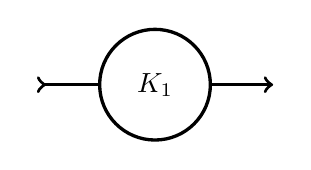
\begin{tikzpicture}[every path/.style={very thick}]
          \node[draw,circle,minimum size=40pt] (A) at (0,0) {$K_1$};
          \node (L) at (-1.5,0) {};
          \node (R) at (1.5,0) {};

          \draw[>-] (L.center) -- (A);
          \draw[->] (A) -- (R.center);
        \end{tikzpicture}
      \end{aligned} \times
      \begin{aligned}
        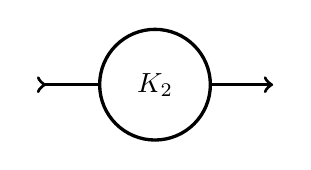
\begin{tikzpicture}[every path/.style={very thick}]
          \node[draw,circle,minimum size=40pt] (A) at (0,0) {$K_2$};
          \node (L) at (-1.5,0) {};
          \node (R) at (1.5,0) {};

          \draw[>-] (L.center) -- (A);
          \draw[->] (A) -- (R.center);
        \end{tikzpicture}
      \end{aligned} =
      \begin{aligned}
        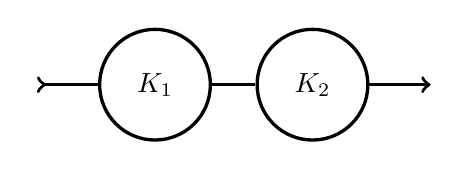
\begin{tikzpicture}[every path/.style={very thick}]
          \node[draw,circle,minimum size=40pt] (A) at (0,0) {$K_1$};
          \node[draw,circle,minimum size=40pt] (B) at (2,0) {$K_2$};
          \node (L) at (-1.5,0) {};
          \node (R) at (3.5,0) {};

          \draw[>-] (L.center) -- (A);
          \draw (A) -- (B);
          \draw[->] (B) -- (R.center);
        \end{tikzpicture}
      \end{aligned}
      \]
      \caption{The two-leg sum operation $\times$. If both $A$ and $B$ are two-leg-prime, then $A \times B$ has
        exactly one separating edge.}
      \label{fig:legsum_example}
    \end{figure}
    Hence, we will take $\ArbSubClass$ to be the class of knot shadows
    which remain at least 2-connected after removing the root edge.

    Certainly $A \times B \in \KnotShad$ as we obtain a new 2-leg shadow. As $\times$ introduces no
    crossings, we have $k = 0$ and $|A \times B| = |A| + |B|$. Finally, a 2-leg shadow $K$ either lies in
    $\ArbSubClass$ or has $\ell-1$ disconnecting edges. Cutting these edges produces the disjoint
    union of $\ell$ well-ordered 2-leg shadows (well ordered from their position in the long curve $K$)
    which is the unique ordered $+$-decomposition of $K$ into elements of $\ArbSubClass$.

    Let $\varphi$ be the map which twists the root edge, making the loop the new root (using the
    appropriate induced orientation). Then $\varphi: \KnotShad_* \hookrightarrow \ArbSubClass_{*+1}$,
    since deleting the root and smoothing the pointed edge produces a knot shadow, which must be at
    least 2-connected.
    \begin{figure}[h!]  \centering
      \[
      \begin{aligned}
        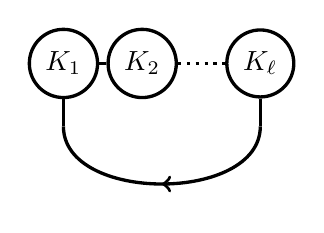
\begin{tikzpicture}[every path/.style={very thick},decoration={markings, mark=at position 0.5 with {\arrow{>}}}]
          \node[draw,circle,minimum size=15pt] (A) at (0,0) {$K_1$};
          \node[draw,circle,minimum size=15pt] (B) at (1,0) {$K_2$};
          \node[draw,circle,minimum size=15pt] (C) at (2.5,0) {$K_\ell$};
          \node (L) at (0,-.8) {};
          \node (R) at (2.5,-.8) {};

          \draw (L.center) -- (A);
          \draw (A) -- (B);
          \draw[dotted] (B) -- (C);
          \draw (C) -- (R.center);
          \draw (R.center) edge[out=-90,in=-90,postaction={decorate}] (L.center);
        \end{tikzpicture}
      \end{aligned} \xmapsto{\varphi}
      \begin{aligned}
        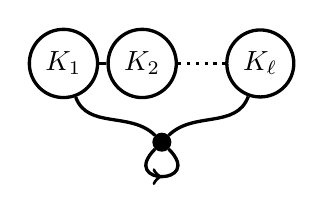
\begin{tikzpicture}[every path/.style={very thick},decoration={markings, mark=at position 0.5 with
        {\arrow{>}}}]
          \node[draw,circle,minimum size=15pt] (A) at (0,0) {$K_1$};
          \node[draw,circle,minimum size=15pt] (B) at (1,0) {$K_2$};
          \node[draw,circle,minimum size=15pt] (C) at (2.5,0) {$K_\ell$};
          \node[draw,circle,fill=black,inner sep=2pt] (X) at (1.25,-1) {};

          \draw (X) edge[in=-70,out=90+45] (A);
          \draw (A) -- (B);
          \draw[dotted] (B) -- (C);
          \draw (C) edge[out=-110,in=90-45] (X);
          \draw (X) edge[out=-135,in=-45,postaction={decorate},looseness=10] (X);
        \end{tikzpicture}
      \end{aligned} \xmapsto{\varphi}
      \begin{aligned}
        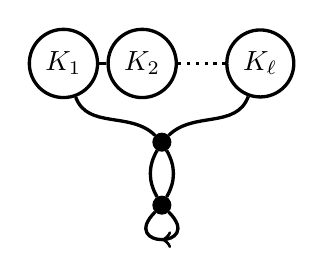
\begin{tikzpicture}[every path/.style={very thick},decoration={markings, mark=at position 0.5 with
            {\arrow{>}}}]
          \node[draw,circle,minimum size=15pt] (A) at (0,0) {$K_1$};
          \node[draw,circle,minimum size=15pt] (B) at (1,0) {$K_2$};
          \node[draw,circle,minimum size=15pt] (C) at (2.5,0) {$K_\ell$};
          \node[draw,circle,fill=black,inner sep=2pt] (X) at (1.25,-1) {};
          \node[draw,circle,fill=black,inner sep=2pt] (Y) at (1.25,-1.8) {};

          \draw (X) edge[in=-70,out=90+45] (A);
          \draw (A) -- (B);
          \draw[dotted] (B) -- (C);
          \draw (C) edge[out=-110,in=90-45] (X);
          \draw (X) edge[bend right] (Y);
          \draw (X) edge[bend left] (Y);
          \draw (Y) edge[out=-45,in=-135,postaction={decorate},looseness=10] (Y);
        \end{tikzpicture}
      \end{aligned}
      \]
      \caption{The map $\varphi$ adds a vertex and ensures that the new map is 2-leg-prime.}
      \label{fig:phi_e xample}
    \end{figure}
    Then we take $\psi_0 = \varphi$ and $\psi_1 = \varphi^2$. This setup satisfies the hypotheses
    and hence proves the theorem.
\end{proof}

\begin{corollary}
  There exists $N \ge 0$ and a constant $d < 1$ so that for $n \ge N$,
  \[\Prb(\text{a knot diagram $K$ is an unknot}) < d^n.\]

  For any prime 2-tangle $P$, there exists $N \ge 0$ and constants $d < 1$, $c > 0$ so that for
  $n \ge N$,
  \[\Prb(\text{a knot diagram $K$ contains $\le cn$ copies of $P$ as
    connect summands}) < d^n.\]
  \label{thr:patternthm}
\end{corollary}

\begin{proof}
  The first statement will follow immediately from the second, given a
  prime 2-tangle corresponding to a prime knot diagram which is not an
  unknot. The second is a corollary of
  theorems~\ref{thr:strongpattern} and~\ref{thr:smoothgrowth}: Let $P$
  be a prime 2-tangle which can be found as a connect summand of a knot
  diagram (i.e., it has one link component). If $m_n$ is the number of
  knot diagrams, then there exists $c > 0$, $d > 1$, and $N > 0$ so
  that for all $n \ge N$, $\frac {h_n}{m_n} < d^n$, where $h_n$ is the
  number of knot diagrams which contain at most $cn$ copies of $P$ as
  connect summands. This ratio is precisely the probability in the
  second statement.
\end{proof}

\subsubsection{Smooth growth for prime knot and link diagrams}
\label{sec:smoothprime}

If, however, we are considering a class $\PrimeShad$ of prime or
reduced rooted diagrams, the method of proof for smoothness does not
immediately carry over; it is possible that $\varphi$ introduces
numerous isthmi, in which case our diagrams created in the final step
would not even be reduced. In the case where $\PrimeShad$ is the class
of prime rooted link shadows, exact counts are known from their
bijection with simple quadrangulations~\cite{AlbenqueSQT};
\[ s_n = \frac{4(3n)!}{n!(2n + 2)!}.\]
In other cases again smoothness is more complicated to prove, although we can use a similar argument
to that in the case of all knot shadows.

\begin{proposition}
  Prime knots
\end{proposition}

\begin{proof}
  Step i is again immediate, so we begin with step ii. Let $\psi, \psi'$ respectively be maps which
  take the root vertex to the two 4-tangle shadows:

  Observe that neither $\psi$ nor $\psi'$ remove primeness or reducedness. Their images provide an
  injection into the spaces with 2 and 3 additional crossings, respectively. So take $m$
  appropriately.

  Define the operation $+$ now by the detour-glom. Notice that primeness is preserved and the
  process is splittable; given the root edge we can identify the bendy edges and rebuild the old two
  shadows. Notice that $|A + B| = |A| + |B| + 4$. Now let $C_3 \ge 1$ and $C_2 = C_3(r +
  \delta)^{-4}$. Then if there exist nonnegative integers $a, b$ such that $n = am + b(m+1) + (a+b)4
  = a(m + 4) + b(m+5)$, i.e.\ if $n \ge (m+4)(m+5)$, then
  \[ p_n > p_{m+4}^ap_{m+5}^b > C_2^{a+b}(r+\delta)^{-(am+b(m+1))} > C_3^{a+b}(r+\delta)^{-(a(m+4) + b(m+5))}
  > C_3(r+\delta)^{-n}.\]
\end{proof}

\subsubsection{Proof and constructions for the pattern theorem}
\label{sec:proof-patt}

The crux of applying this theorem to link diagrams then falls upon
determining an ``attachment'' operation which satisfies the
hypotheses, along with patterns valid for a given class of shadows.
We can generally define attachment operations for different kinds of
tangles in the dual. By abuse of notation, let $S = (\{0\}, \{0\}, S)$ be a set of
labels for the faces of the dual (for now, we are concerned about
diagrams, which only have labeled vertices).
\begin{enumerate}
\item \textbf{Connect sum.} Let $L$ and $Q'$ be rooted $S$-quadrangulations. Orient the
  remaining edges of $L$ canonically by proposition~\ref{prop:canonicalori}. Define the
  \emph{connect sum} of $Q'$ into $L$ at an edge $e \in L$, $L \#_e Q'$, by
  \begin{enumerate}
  \item Cut and split the edge $e$, creating a map $L'$ and leaving a distinguished, oriented bigon
    $f$. Denote the two edges formed by splitting $e$ by $e_1$, $e_2$, so that the loop $e_1(-e_2)$
    is a counterclockwise cycle around $f$. If $e$ was the root of $L$, make $e_1$ the new root of
    $L'$.
  \item Cut and split the root edge $\epsilon$ of $Q'$, creating a map $Q$ and leaving a
    distinguished, oriented bigon $g$. Denote the two edges formed by splitting $\epsilon$ by
    $\epsilon_1, \epsilon_2$, so that the loop $\epsilon_1(-\epsilon_2)$ is a counterclockwise cycle
    around $g$. Make $\epsilon_2$ the new root of $Q$.
  \item Glue the map $Q$ into the map $L'$'s distinguished face $f$ along the boundary of the
    distinguished bigon $g$ so that $e_1$ and $\epsilon_2$ are mapped to the same edge and so that
    the orientations of the boundaries align.
  \item Forget about all edge orientations except for the root edge of $L$.
  \end{enumerate} Notice that none of the original faces in $L$ and $Q'$ are changed; hence the
  result is a new rooted $S$-quadrangulation. Any given $S$-quadrangulation in $2n$ edges
  has precisely $2n$ different non-conflicting sites for connect summation (i.e. $k = 1$ for this
  attachment operation). This process is reversible, given a 2-cycle which bounds an instance of
  $Q'$ (collapse the disk to a single edge).
  \begin{figure}[h!]  \centering
    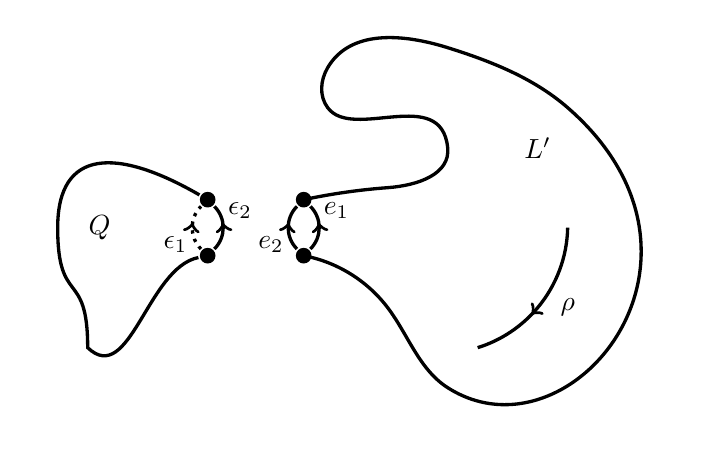
\begin{tikzpicture}
      % \node[anchor=south west, inner sep=0] (img) at (0,0)
      % {\includegraphics[height=2in]{connect_sum_topology}};x={(img.south east)},y={(img.north
      % west)},
      \begin{scope}[x={(3in,0in)},y={(0in,2in)},every
        node/.style={circle,fill=black,inner sep=2pt},every
        path/.style={black,very thick},decoration={markings, mark=at position
          0.6 with {\arrow{>}}}]
        % \draw[help lines,xstep=.1,ystep=.1] (0,0) grid (1.1,1);
        \useasboundingbox (0,0) rectangle (1.1,1);
        \node (L_A) at (.46,.43) {};
        \node (L_B) at (.46,.57) {};
        \draw[out=90+45,in=180+45,postaction={decorate}] (L_A) to node[fill=none,midway,below left]{$e_2$} (L_B);
        \draw[out=90-45,in=-45,postaction={decorate}] (L_A) to node[fill=none,midway,above
        right]{$e_1$} (L_B);
        \node[fill=none] (L_L') at (.85,.7) {$L'$};
        \draw[hobby,postaction={decorate}] plot coordinates {(.9,.5) (.85,.3) (.75,.2)};
        \node[fill=none] (root) at (.9,.3) {$\rho$};


        % \draw (L_B) .. controls (.7,.6) and (.7,.75) .. (.6,.8)
        % .. controls +(130:.2) and +(270:.1) ..
        % (.5,.9) -- (.9,.9) -- (.9,.2) -- (L_A);
        \draw[hobby] plot coordinates {(L_B) (.6,.6) (.7,.7) (.5,.8)
          (.5,.9) (.7,.95) (.9,.8) (.7,.1) (.6,.3) (L_A)};

        \node (Q_A) at (.3,.43) {};
        \node (Q_B) at (.3,.57) {};
        \draw[out=90-45,in=-45,postaction={decorate}] (Q_A) to node[fill=none,midway,above right]{$\epsilon_2$} (Q_B);
        \draw[dotted,out=90+45,in=180+45,postaction={decorate}] (Q_A) to
        node[fill=none,midway,below left]{$\epsilon_1$} (Q_B);
        \draw (Q_B) .. controls (.15,.7) and (.05,.7) .. (0.05,.5)
        .. controls (.05,.3) and (.1,.4) .. (.1,.2) .. controls
        (.17,.1) and (.2,.4) .. (Q_A);
        \node[fill=none] (Q_Q') at (.12,.5) {$Q$};

      \end{scope}
    \end{tikzpicture}
    \caption{The connect sum operation. $Q'$ and $L'$ are viewed as CW-complexes, and their
      boundaries are appropriately identified.}
    \label{fig:cs_topology}
  \end{figure}
  If $L^*$ and $(Q')^*$ each consist of only one link component, then
  $(L\#_eQ')^* =: L^*\#_e(Q')^*$ will as well. In fact, this
  attachment into the quadrangulation is precisely dual to the usual
  link connect sum from knot theory. If $Q$ is 2-leg prime, then no
  two copies of $Q$ can intersect (as in this case there are precisely
  two paths of length 1 in $Q$ between its two boundary vertices).

\item \textbf{4-tangle replacement.} Let $L$ be a rooted
  $S$-quadrangulation, and $Q$ a rooted $S$-quadrangulation with
  square boundary. Then given a face $f \in L$, we can define a
  \emph{4-tangle replacement} of $f$ with $Q$ by identifying the
  boundary of $Q$ with the boundary of $f$ in some manner. Precisely
  how to equate the boundaries will depend on the case at hand; what
  matters is that there be at least one valid way to glue $Q$ into any
  face $f$ and produce a new $S$-quadrangulation in the chosen
  class. Indeed, the result will always be a new
  $S$-quadrangulation. Any $S$-quadrangulation in $2n$ edges has $n$ faces, and hence at
  least $n$ non-conflicting attachment locations (i.e., $k = 2$).

  To make the process reversible for all $S$ (not just $S = \{0\}$),
  we must pick slightly different $Q$. Given a non-trivial $S$-map
  $P$, choose a planar rooted labeled map with boundary $Q$ which cannot
  intersect with a copy of itself so that $P$ is a unique copy of
  itself in $Q$, where all faces which are not in $P$ are labeled
  with a special label $*$. Attachment of $Q$ into the face $f$ of an
  $S$-quadrangulation $L$ then consists first of the actual attachment
  operation described above, and then relabeling all faces with label
  $*$ with the original label of $f$. The process is then reversed by
  \begin{enumerate}
  \item Given a 4-cycle bounding a (relabeled) copy $Q'$ of $Q$ in
    $L$, tentatively delete the copy and replace it with a bare face
    $f$.
  \item Identify the unique copy of $P$ inside of $Q$.
  \item If every face of $Q \setminus P$ does not have the same
    label $x$, then this would not in fact have been a place of attachment
    (hence reversal needn't be possible). If they do, then label the
    new face $f$ with the label $x$.
  \end{enumerate}

  Care must be taken in choice of $Q$ in which to embed arbitrary $P$
  here; an important fact to remember is that submap insertion of any
  $S$-quadrangulation with boundary $P$ will not introduce any shorter
  paths through $Q$, else there would be a $3$-cycle in $P$ (which is
  impossible as it is a quadrangulation).

  If one is dealing with 4-tangle replacement within a class of knot
  $S$-shadow duals, the following lemma is helpful;
  \begin{lemma}
    Given a link $S$-shadow $L$, a vertex $v$ in $L$, and an 4-leg
    $S$-curve $T$ with 2 link components, it is always possible to
    replace $v$ by $T$ in at least one way so that the result has the
    same number of components as $L$.
  \end{lemma}
  \begin{proof}
    TODO: This proof needs work

    The vertex $v$ in $L$ and the tangle $T$ are each either of
    crossing (abab) type or tangency (aabb) type. If they agree in
    type, replace $v$ by $T$ so that the strands agree. If they differ
    and $L \setminus v$ is of type abab, replace $T$ in with type
    abba. If they differ and $L \setminus v$ is of type aabb, replace
    $T$ with type abab. In all cases, the number of components is
    preserved.
  \end{proof}


  There are applications of this attachment in proving the weak
  pattern theorem for certain classes of maps:
  \begin{enumerate}[i.]
  \item Given arbitrary face labels $S$, a prime link dual $S$-shadow $L$
    and a prime 4-leg dual $S$-curve $P$,
    define $Q$ as in figure~\ref{fig:linktangrep}.
    \begin{figure}[h!]
      \centering
      % \includegraphics[width=2in]{dual_to_fig8twist}
      \begin{tikzpicture}[every path/.style={string, thick, gray}, every node/.style={transform shape,
          knot crossing, circle, fill=gray, inner sep=2pt}]
        \begin{scope}
          % \draw[red,step=.5] (-2,-2) grid (2,2);
          \useasboundingbox (-2,-2) rectangle (2,2);
          \node[fill=none,draw=gray,minimum size=20pt] (O) at (0,0) {};
          \node[fill=none] (LL) at (-2,0) {};
          \node (L) at (-1,0){};
          \node (R) at (1,0) {};
          \node[fill=none] (RR) at (2,0) {};
          \node[fill=none] (UU) at (0,2) {};
          \node (U) at (0,1) {};
          \node (D) at (0,-1) {};
          \node[fill=none] (DD) at (0,-2) {};

          \draw (LL) -- (L) -- (O) -- (R) -- (RR);
          \draw (UU) -- (U) -- (O) -- (D) -- (DD);
          \draw (L) edge[out=90,in=180] (U);
          \draw (U) edge[out=0,in=90] (R);
          \draw (R) edge[out=-90,in=0] (D);
          \draw (D) edge[out=180,in=-90] (L);
        \end{scope}
        \begin{scope}[every path/.style={string, very thick, black}, every
          node/.style={transform shape, knot crossing, circle, fill=black,
            inner sep=2pt}, decoration={markings, mark=at position 0.4 with
            {\arrow{<}}}]
          \useasboundingbox (-2,-2) rectangle (2,2);
          \node (a) at (-1.5,1.5) {};
          \node (b) at (1.5,1.5) {};
          \node (c) at (1.5,-1.5) {};
          \node (d) at (-1.5,-1.5) {};
          \draw (a) -- (b) -- (c);
          \draw[postaction={decorate}] (c) -- (d);
          \draw (d) -- (a);

          \node (e) at (-.5,.5) {};
          \node (f) at (.5,.5) {};
          \node (g) at (.5,-.5) {};
          \node (h) at (-.5,-.5) {};
          \draw (e) -- (f) -- (g) -- (h) -- (e);

          \draw (a) -- (e);
          \draw (b) -- (f);
          \draw (c) -- (g);
          \draw (d) -- (h);

          \node[fill=none,draw=none] (P) at (0,0) {$P$};
        \end{scope}
      \end{tikzpicture}
      \caption{The labeled quadrangulation $Q$ (in black) is dual to
        encircling the 4-leg curve $P$ with a link component. The four
        faces bounding $P$ have the distinguished label $*$.}
      \label{fig:linktangrep}
    \end{figure}
    Observe that if there exist two copies $Q'$ and $Q''$ of $Q$ in a
    prime link dual shadow $L$, then they cannot intersect: All paths
    between boundary vertices of $Q$ are either of length $3$, or
    greater. If there is an intersection between $Q'$ and $Q''$, then
    without loss of generality one of two things happens: (1) There is
    a path along the root face of $Q''$ of 3 edges lies in $Q'$ (since
    there are no paths of length 1 or 2) and runs between two adjacent
    vertices $a$ and $b$ of $Q'$; but then the remaining boundary edge
    of $Q''$ must run from $a$ to $b$; but this gives the existence of
    a 2-cycle in $L$ which we said was prime and hence has no
    2-cycles. (2) The entire boundary cycle of $Q''$ lies within $Q'$
    and necessarily runs between two opposing vertices $a$ and $c$ of
    $Q'$. But then these two opposing vertices must be the same vertex
    in $L$; but then there is the 2-cycle $a$ to $b$ to $c=a$ in $L$,
    which again was chosen to have no 2-cycles.
  \item Given face labels $S$, a prime \emph{knot} dual $S$-shadow
    $K$, and a nontrivial prime 4-leg dual $S$-curve with $2$ components $P$,
    define $Q$ as in figure \ref{fig:knottangrep}, embedding $P$ in
    such a way that $Q$ has precisely 2 link components.
    \begin{figure}[h!]
      \centering
      % \includegraphics[width=2in]{dual_to_fig8twist}
      \begin{tikzpicture}[every path/.style={string, thick, gray}, every node/.style={transform shape,
          knot crossing, circle, fill=gray, inner sep=2pt}]
        \begin{scope}
          % \draw[red,step=.5] (-2,-2) grid (2,2);
          \useasboundingbox (-2,-2) rectangle (2,2);
          \node[fill=none,draw=gray,minimum size=15pt] (O) at (.4,.4) {};
          \node (Q) at (-.4,-.4) {};
          \node (K) at (.4,-.4) {};

          \node[fill=none] (LL) at (-2,0) {};
          \node (L) at (-1.15,-.2){};
          \node (R) at (1.15,.4) {};
          \node[fill=none] (RR) at (2,0) {};
          \node[fill=none] (UU) at (0,2) {};
          \node (U) at (.2,1.15) {};
          \node (D) at (-.4,-1.15) {};
          \node[fill=none] (DD) at (0,-2) {};

          \draw (LL) -- (L) -- (Q) -- (K) edge[out=0, in=-90] (R);
          \draw (R) edge[out=90, in=0,looseness=1.5] (U);
          \draw (U) edge[out=180,in=90,looseness=1.8] (L);
          \draw (L) edge[out=-90,in=180,looseness=1.5] (D);
          \draw (UU) -- (U) -- (O) edge[out=180,in=90] (Q);
          \draw (O) -- (R) -- (RR);
          \draw (D) edge[out=0,in=-90] (K);
          \draw (K) -- (O);
          \draw (Q) -- (D) -- (DD);
        \end{scope}
        \begin{scope}[every path/.style={string, very thick, black}, every
          node/.style={transform shape, knot crossing, circle, fill=black,
            inner sep=2pt}, decoration={markings, mark=at position 0.4 with
            {\arrow{<}}}]
          \useasboundingbox (-2,-2) rectangle (2,2);
          \node (a) at (-1.5,1.5) {};
          \node (b) at (1.5,1.5) {};
          \node (c) at (1.5,-1.5) {};
          \node (d) at (-1.5,-1.5) {};
          \draw (a) -- (b) -- (c);
          \draw[postaction={decorate}] (c) -- (d);
          \draw (d) -- (a);

          \node (e) at (-.8,.8) {};
          \node (f) at (.8,.8) {};
          \node (g) at (.8,0) {};
          \node (h) at (0,0) {};
          \node (i) at (0,-.8) {};
          \node (j) at (-.8,-.8) {};

          \draw (e) -- (f) -- (g) -- (h) -- (i) -- (j) -- (e);
          \draw (e) -- (h);

          \draw (a) -- (e);
          \draw (b) -- (f);
          \draw (i) -- (c) -- (g);
          \draw (d) -- (j);

          \node[fill=none,draw=none] (P) at (.4,.4) {$P$};
        \end{scope}
      \end{tikzpicture}
      \caption{The labeled quadrangulation $Q$ (in black) in which to
        embed $P$. The remaining
        faces bounding $P$ have the distinguished label $*$.}
      \label{fig:knottangrep}
    \end{figure}
    Observe that, as in the case above, the shortest paths which both
    start and end on the boundary of $Q$ are of length 3 between
    adjacent vertices, or length 4 between opposite vertices. As we
    are taking $K$ to be prime, the same reasoning shows that copies
    of $Q$ in $K$ can not overlap. On the other hand, we must now be
    careful that the 4-tangle replacement into a knot dual $S$-shadow
    does not introduce new link components. Fortunately, there is
    always at least one way to insert a 4-leg dual $S$-curve while
    keeping constant the number of link components.
  \end{enumerate}
\end{enumerate}

\subsubsection{Strategy for proving smooth growth}
\label{sec:smoothstratproof}


\subsection{Asymmetry of diagrams and consequences}
\label{sec:asymmetry}


The following theorem of Richmond and Wormald \cite{Richmond19951} provides a sufficient set of
criteria for almost all elements of $\FlatKnotDia$ to have trivial automorphism group.

\begin{theorem}[Richmond-Wormald 1996]
  Let $\mathscr C$ be a class of rooted maps on a surface. Suppose that there is an outer-cyclic
  rooted planar map $M_1$ such that in all maps in $\mathscr C$, all copies of $M_1$ are pairwise
  disjoint, and such that
  \begin{enumerate}
  \item $M_1$ has no reflective symmetry in the plane preserving the unbounded face,
  \item there exist constants $c > 0$ and $d < 1$ such that the proportion of $n$-vertex maps in
    $\mathscr C$ that do not contain at least $cn$ pairwise disjoint copies of $M_1$ is at most
    $d^n$ for $n$ sufficiently large ($M$ is ``ubiquitous''), and
  \item for any map $M$ in $\mathscr C$ containing a copy of $M_1$, all maps obtainable by removing
    $M_1$ and gluing it back in to the same face are in $\mathscr C$ ($M$ is ``free'').
  \end{enumerate}
  Then the proportion of $n$-vertex maps in $\mathscr C$ with nontrivial automorphisms is
  exponentially small.
\end{theorem}

It has been suggested without proof in~\cite{zuber2015mapsimsperms,pzjschaeff2004planecurveasymp} that classes of knot shadows
are almost surely asymmetric. We will prove this for $\FlatKnotDia$ by
proving it for its dual $\FlatKnotDia^*$, a class of quadrangulations
of the sphere. Specifically, we will take $M_1$ to be the dual of the
underlying planar map of the following 2-tangle:
\begin{figure}[h!]
  \centering
  \begin{tikzpicture}
    \begin{scope}
    [every path/.style={string, thick, gray}, every node/.style={transform shape,
      knot crossing, inner sep=1.5pt}]
    %\draw[help lines,step=.5] (-3,-2) grid (3, 3);
    \node (a) at (-1.5,.5) {};
    \node (b) at (1,0) {};

    \node (x) at (-1,1) {};
    \node (y) at (.5,1.5) {};
    \node (z) at (.25,.7) {};

    \node (el) at (-2.7,0) {};
    \node (er) at (2.7,0) {};

    \draw[>-] (el.center) .. controls (el.4 east) and (a.4 south west) .. (a);

    \draw (a) -- (x.center);
    \draw (x.center) .. controls (x.8 north east)  and (y.4 north west)  .. (y);
    \draw (y)        .. controls (y.16 south east) and (z.2 east)        .. (z.center);
    \draw (z.center) .. controls (z.2 west)        and (x.4 south east)  .. (x);
    \draw (x)        .. controls (x.16 north west) and (a.8 north west)  .. (a.center);
    \draw (a.center) .. controls (a.16 south east) and (b.16 south west) .. (b);
    \draw (b)        .. controls (b.32 north east) and (y.4 north east)  .. (y.center);
    \draw (y.center) .. controls (y.8 south west)  and (z.2 north)       .. (z);
    \draw (z)        .. controls (z.2 south)       and (b.4 north west)  .. (b.center);

    \draw[->] (b.center) .. controls (b.4 south east) and (er.4 west) .. (er.center);
  \end{scope}
  \begin{scope}[every path/.style={very thick}, every node/.style={circle,fill=black, inner sep=2pt}]
    \node (T) at (0,2.5) {};
    \node (B) at (0,-1) {};

    \node (X) at (-1.5, 1) {};
    \node (Y) at (-.5,1) {};
    \node (Z) at (.5, 1) {};
    \node (W) at (1.5, 1) {};

    \node (O) at (0,0) {};

    \path (T) edge (X)
               edge (Y)
               edge (W)
          (O)  edge (X)
               edge (Y)
               edge (W)
               edge (B)
          (Z)  edge (Y)
               edge (W);

    \draw (T) .. controls (-3,2) and (-3,-.5) .. (B);
    \draw (T) .. controls (3,2) and (3,-.5) .. (B);
  \end{scope}
  \end{tikzpicture}
  \caption{The dual 2-leg curve $M_1$ (black), and one of its representations as
    a 2-tangle (gray).}
  \label{fig:treflegs2}
\end{figure}
Clearly $M_1$ has no reflective symmetry by inspection, and certainly
any of the ways of replacing $M_1$ keep the object in the class of
quadrangulations dual to knot maps. Finally, the ubiquity condition is
exactly the pattern theorem for 2-tangles proved in the prior section!
The same pattern proves asymmetry for certain other classes of knots
or links; for example, reduced diagrams.

Additionally, we can use our 4-tangle replacement scheme to create a
$M_1$ which shows asymmetry of prime knot (link) diagrams. Take $M_1$
as in figure~\ref{fig:primeknotasymm}.
\begin{figure}[h!]
  \centering
  % \includegraphics[width=2in]{dual_to_fig8twist}
  \begin{tikzpicture}
    \begin{scope}[every path/.style={string, thick, gray}, every node/.style={transform shape,
        knot crossing, circle, fill=gray, inner sep=1.5pt}]
      % \draw[red,step=.5] (-2,-2) grid (2,2);
      \useasboundingbox (-2,-2) rectangle (2,2);
      \node (O) at (.6,.6) {};
      \node (O2) at (.1,.25) {};
      \node (Q) at (-.4,-.4) {};
      \node (K) at (.4,-.4) {};

      \node[fill=none] (LL) at (-2,0) {};
      \node (L) at (-1.15,-.2){};
      \node (R) at (1.15,.4) {};
      \node[fill=none] (RR) at (2,0) {};
      \node[fill=none] (UU) at (0,2) {};
      \node (U) at (.2,1.15) {};
      \node (D) at (-.4,-1.15) {};
      \node[fill=none] (DD) at (0,-2) {};

      \draw (LL) -- (L) -- (Q) -- (K) edge[out=0, in=-90] (R);
      \draw (R) edge[out=90, in=0,looseness=1.5] (U);
      \draw (U) edge[out=180,in=90,looseness=1.8] (L);
      \draw (L) edge[out=-90,in=180,looseness=1.5] (D);
      \draw (UU) -- (U) -- (O) edge[out=180,in=90,looseness=1.5] (O2);
      \draw (O) -- (R) -- (RR);
      \draw (D) edge[out=0,in=-90] (K);
      \draw (O) edge[out=-90,in=0,looseness=1.8] (O2);
      \draw (O2) -- (K);
      \draw (Q) edge[out=90, in=190,looseness=1.8] (O2);
      \draw (Q) -- (D) -- (DD);
    \end{scope}
    \begin{scope}[every path/.style={string, very thick, black}, every
      node/.style={transform shape, knot crossing, circle, fill=black,
        inner sep=2pt}, decoration={markings, mark=at position 0.4 with
        {\arrow{<}}}]
      \useasboundingbox (-2,-2) rectangle (2,2);
      \node (a) at (-1.5,1.5) {};
      \node (b) at (1.5,1.5) {};
      \node (c) at (1.5,-1.5) {};
      \node (d) at (-1.5,-1.5) {};
      \draw (a) -- (b) -- (c);
      \draw (c) -- (d);
      \draw (d) -- (a);

      \node (e) at (-.8,.8) {};
      \node (f) at (.8,.8) {};
      \node (g) at (.8,0) {};
      \node (h) at (0,0) {};
      \node (i) at (0,-.8) {};
      \node (j) at (-.8,-.8) {};

      \node (x) at (.4,.4) {};

      \draw (e) -- (f) -- (g) -- (h) -- (i) -- (j) -- (e);
      \draw (e) -- (h);

      \draw (a) -- (e);
      \draw (b) -- (f);
      \draw (i) -- (c) -- (g);
      \draw (d) -- (j);

      \draw (e) -- (x) -- (g);

    \end{scope}
  \end{tikzpicture}
  \caption{Choice of $M_1$ for proving that prime knot shadows
    are asymmetric}
  \label{fig:primeknotasymm}
\end{figure}
Then $M_1$ consists of exactly two link components and is of abab
type; any way of replacing a vertex in a knot shadow with a 4-leg
curve of abab type keeps the number of link components
constant. Furthermore, $M_1$ is ubiquitous in prime (knot) diagrams as
it is an application of corollary~\ref{thr:patternthm} to $P$, the
square with an additional 2-path joining two of its opposite vertices.

Application of the above theorems provides us with the following corollary which enables us to
transfer any asymptotic results on rooted diagrams to unrooted diagrams.

\begin{corollary}
  Let $L$ be a uniform random variable taking values in the space $\KnotDia_n$ or $\LinkDia_n$. Then
  there exist constants $C, \alpha > 0$ so that $\Prb(\Aut L \ne 1) < Ce^{-\alpha n}$. Hence, rooted
  diagrams behave like unrooted diagrams.
\end{corollary}

Indeed, link diagrams with $n$ vertices are dual to quadrangulations with $n+2$ faces; there are
$n+2$ ways of choosing the ``exterior'' root face and then $4$ ways of rooting the edges around this
chosen face. Hence if $\tilde \ell_n$, $\tilde k_n$ are the counts of unrooted link or knot diagrams
we have that in the limit,
\[ \tilde\ell_n \underset{n\to\infty}{\sim} \frac{\ell_n}{4(n+2)} \text{ and } \tilde k_n
\underset{n\to\infty}{\sim} \frac{k_n}{4(n+2)}.\]

\begin{corollary}
  A random knot or link diagram has the pattern theorem. Namely, a random knot diagram is almost
  surely composite and almost surely knotted, and a random link diagram is almost surely not a knot
  diagram.
\end{corollary}

\section{Some numerical results}
\label{sec:randres}

[[Blurb about pattern appearances; counts of monogons in diagrams]]

One may be concerned that the ``asymptotic'' behavior proved in the prior section only applies to
knot diagrams with an absurd number of crossings (in the sense that no physical knot should be
expected to be so complicated). However, exact and numerical results show that this behavior is
attained very quickly. For example, almost all 10-crossing knot diagrams have no nontrivial
automorphisms!

\printbibliography

\end{document}

%%% Local Variables:
%%% mode: latex
%%% TeX-master: t
%%% End:
